\documentclass[a4paper,10pt,ngerman]{scrartcl}
\usepackage{babel}
\usepackage[T1]{fontenc}
\usepackage[utf8x]{inputenc}
\usepackage[a4paper,margin=2.5cm,footskip=0.5cm]{geometry}

\newcommand{\Aufgabe}{Aufgabe 2: Simultane Labyrinthe}
\newcommand{\TeilnahmeId}{76626}                 
\newcommand{\Name}{Quirin Klemm}            


% Kopf- und Fußzeilen
\usepackage{scrlayer-scrpage, lastpage}
\setkomafont{pageheadfoot}{\large\textrm}
\lohead{\Aufgabe}
\rohead{Teilnahme-ID: \TeilnahmeId}
\cfoot*{\thepage{}/\pageref{LastPage}}

% Position des Titels
\usepackage{titling}
\setlength{\droptitle}{-1.0cm}

% Für mathematische Befehle und Symbole
\usepackage{amsmath}
\usepackage{amssymb}

% Für Bilder
\usepackage{graphicx}

% Für Algorithmen
\usepackage{algpseudocode}

% Für Quelltext
\usepackage{listings}
\usepackage{color}
\definecolor{mygreen}{rgb}{0,0.6,0}
\definecolor{mygray}{rgb}{0.5,0.5,0.5}
\definecolor{mymauve}{rgb}{0.58,0,0.82}
\lstset{
  keywordstyle=\color{blue},commentstyle=\color{mygreen},
  stringstyle=\color{mymauve},rulecolor=\color{black},
  basicstyle=\footnotesize\ttfamily,numberstyle=\tiny\color{mygray},
  captionpos=b, % sets the caption-position to bottom
  keepspaces=true, % keeps spaces in text
  numbers=left, numbersep=5pt, showspaces=false,showstringspaces=true,
  showtabs=false, stepnumber=2, tabsize=2, title=\lstname
}
\lstdefinelanguage{JavaScript}{ % JavaScript ist als einzige Sprache noch nicht vordefiniert
  keywords={break, case, catch, continue, debugger, default, delete, do, else, finally, for, function, if, in, instanceof, new, return, switch, this, throw, try, typeof, var, void, while, with},
  morecomment=[l]{//},
  morecomment=[s]{/*}{*/},
  morestring=[b]',
  morestring=[b]",
  sensitive=true
}

% Diese beiden Pakete müssen zuletzt geladen werden
%\usepackage{hyperref} % Anklickbare Links im Dokument
\usepackage{cleveref}

% Daten für die Titelseite
\title{\textbf{\Huge\Aufgabe}}
\author{\LARGE Teilnahme-ID: \LARGE \TeilnahmeId \\\\
	    \LARGE Bearbeiter/-in dieser Aufgabe: \\ 
	    \LARGE \Name\\\\}
\date{\LARGE\today}

\begin{document}

\maketitle
\tableofcontents

\vspace{0.5cm}

\clearpage
\section{Lösungsidee}
Gesucht ist möglichst kurze Abfolge von Schritten, die beide Labyrinthe löst. Dafür wird zunächst für jedes Labyrinth eine Matrix erstellt (Abbildung \ref{fig:lybnmatrix}),
in der für jede Position ein Kostenwert und eine Richtung gespeichert wird. Die Richtung zeigt den nächsten Schritt in Richtung Ziel an und ist dargestellt als:
\begin{table}[h]
  \centering
  \begin{tabular}{|c|l|}
      \hline
      \textbf{Code} & \textbf{Richtung} \\
      \hline
      0 & Rechts \\
      1 & Links \\
      2 & Oben \\
      3 & Unten \\
      \hline
  \end{tabular}
  \caption{Codierung der Richtungen im Labyrinth}
  \label{tab:richtungscodierung}
\end{table}
\\
Der Kostenwert gibt an, wie viele Schritte bis zum Ziel benötigt werden.\\
Ein Labyrinth mit dazugehöriger Matrix könnte so aussehen:
\begin{figure}[h]
  \centering
  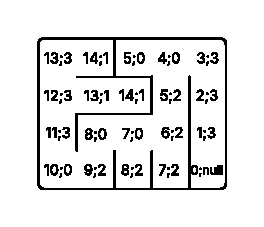
\includegraphics[width=0.4\textwidth]{Simultane Labyrinthe/pdf_src/cost_matrix.pdf}
  \caption{Labyrinth und Matrix}
  \label{fig:lybnmatrix}
\end{figure}

\subsection{Erstellung der Matrix}
Zu Beginn wird eine Matrix erstellt, deren Werte für alle Positionen zunächst leer sind.
Ausgehend vom Zielpunkt durchläuft der Algorithmus rekursiv alle erreichbaren Nachbarpositionen.
Für jeden Nachbarn wird in der Matrix ein Kostenwert eingetragen, der um eins höher ist als der Kostenwert des aktuellen Punkts, sowie die Richtung, aus der der Nachbar erreicht wurde.


\subsection{Lösen der Labyrinthe}
Der Algorithmus funktioniert so, dass er jeweils den momentan besten Weg der Liste der bisherigen Wege entnimmt und diesen um einen weiteren Schritt erweitert.
Den nächsten Schritt ermittelt er, indem er in der Matrix prüft, welchen Schritt die beiden Labyrinthe für ihre jeweilige Position vorschlagen.
Dieser Schritt wird am Ende der bisherigen Schrittfolge angehängt.
Dabei entstehen in der Regel zwei unterschiedliche Wege. Beide werden zur Liste der bisherigen Wege hinzugefügt.
Zur Auswertung der bisherigen Wege, wird diese Rechung angewandt:
\begin{equation}
  \frac{c_b -c_a}{n}
  \label{weg_kosten}
\end{equation}

wobei gilt:\\
-$c_b$ sind die summierten Kosten von beiden Startpositionen\\
-$c_a$ sind die summierten Kosten von beiden aktuellen Positionen\\
-$n$ ist die Anzahl der benötigten Schritte\\
Der Bruch beschreibt also die durchschnittliche Einsparung pro Schritt – dabei ist 2 der maximal erreichbare Wert.
\\
Der Weg mit der höchsten Einsparung gilt dabei als momentan bester Weg.
Nach jeder Interation wird das aktuelle Positionspaar $((x_1, y_1),(x_2, y_2))$ in einem Dictionary gespeichert,
um zu verhinder, dass der Algorithmus die exakt selben Positionen besucht.
Zusätzlich gibt es auch die Begrenzung $l$ ,die festlegt, wie viele unterschiedliche Weg, sortiert nach ihren Kosten, in der Liste gespeichert werden dürfen.
Diese Begrenung beeinflusst maßgeblich  die Laufzeit und Genauigkeit des Algorithmus.
In der Liste dürfen die Wege unterschiedliche Werte für $n$ haben; wichtig ist lediglich, dass ihre Kosten (Gleichung \eqref{weg_kosten}) gering sind.
Der gesamte Ablauf wiederholt sich solange, bis beide im Ziel sind.

\subsection{Gruben}
Gruben werden sowohl in der Kostenmatrix als auch beim Lösen wie normale Felder gesehen. 
Berührt jedoch einer der beiden eine Grube, wird seine Position auf die jeweilige Startposition zurückgesetzt.
Dadurch steigen die gesamt Kosten des Wegs so weit an, dass dieser wegen der Begrenzung $l$ in der Regel aus der Liste der potenziellen Wege entfernt wird.






\clearpage
\section{Umsetzung}
Die Lösung wurde in Python3 geschrieben. Die Eingabetexte werden eingelesen. 
Für beide Labyrinthe werden die horizontalen und vertikalen Wände jeweils in separenten Liste gespeichert.
Auch die Positionen der Gruben werden für jedes Labyrinth in einer eigenen Liste erfasst.

\subsection{Erstellung der Matrix}
Zur Erstellung der Matrix wird die Klasse $cost$ benutzt.
\begin{figure}[h]
  \centering
  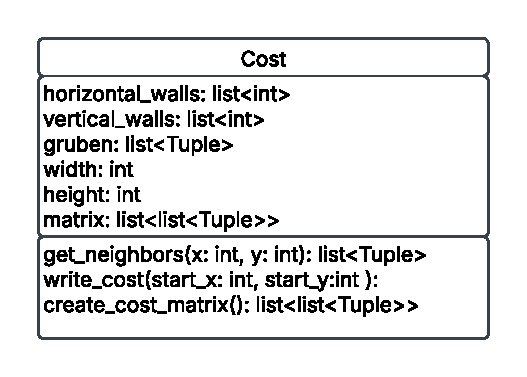
\includegraphics[width=0.6\textwidth]{Simultane Labyrinthe/pdf_src/cost_diagramm.pdf}
  \caption{Cost Klasse}
  \label{fig:cost_diagramm}
\end{figure}
\\
Für jedes Labyrinth wird ein Cost-Objekt erstellt und die Methode
\begin{lstlisting}
  cost_obj.create_cost_matrix()
\end{lstlisting}
\vspace{-2em}
aufgerufen. Das Cost Objekt bekommt als Übergabewerte die horizontalen und vertikalten Wände, die  Gruben sowie die Größe des Labyrinths.
Die $create\_cost\_matrix$ Methode erstellt zunächst eine leere Liste mit der Dimension [height][width], die als Kostenmatrix dient.
Dann ruft sie die Methode $write\_cost$ auf um die Kostenmatrix zufüllen.
\vspace{2em}
\begin{lstlisting}[caption={Methode \texttt{write\_cost}}, label={lst:write_cost}]
  def write_cost(self, start_x: int, start_y: int):
\end{lstlisting}
Zu Beginn wird die Liste $stack$ initalisiert. Sie speichert alle Felder, die noch besucht werden müssen. Die Startposition wird als erstes Element hinzugefügt.
Jeder Eintrag in der Liste besitzt vier Werte: der x-Position, der y-Position, den aktuell Kosten sowie der entgegengesetzen Richtung, aus der das Feld betreten wurde. 
Anschließend wird das erste Element der Liste entnommen und in die Kostenmatrix übertragen.
Falls es schon in der Kostenmatrix ist, wird es übersprungen.
Daraufhin werden alle benachbarten Felder mit der Methode $get\_neighbours$ ermittelt und dem Stack hinzugefügt.
Dabei werden die Kosten um eins erhöht und die jeweilige Richtung gespeichert.
Das wiederholt sich solange bis der Stack leer ist.

\clearpage
\subsection{Lösen der Labyrinthe}

Zum lösen der Labyrinthe wird die Klasse $Solving$ benutzt.
\begin{figure}[h]
  \centering
  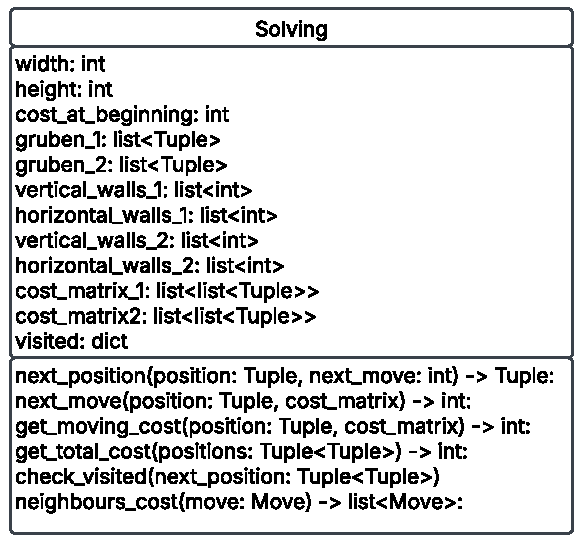
\includegraphics[width=0.6\textwidth]{Simultane Labyrinthe/pdf_src/solving_diagramm.pdf}
  \caption{Solving Klasse}
  \label{fig:solving_diagramm}
\end{figure}

Die Wege werden mit der Klasse $Move$ dargestellt.
\begin{figure}[h]
  \centering
  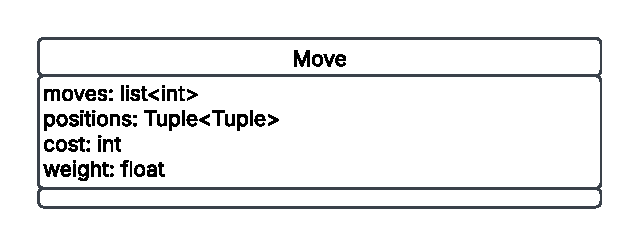
\includegraphics[width=0.6\textwidth]{Simultane Labyrinthe/pdf_src/moving_diagramm.pdf}
  \caption{Moving Klasse}
  \label{fig:moving_diagramm}
\end{figure}
\\
Das Attribut $cost$ beschreibt die aufsummierten Kosten der beiden aktuellen Positionen basierend auf den Werten aus den Kostmatrizen.
Das Attribut $weight$ wird gemäß der Gleichung \eqref{weg_kosten} berechnet.\\
Zu Beginn wird ein $Solving$-Objekt initalisiert und eine leere Liste $moves$ angelegt, in der alle aktuelle Wege gespeichert werden.
Anschließend wird ein erstes $Move$-Objekt erzeugt, dessen Startposition ((0, 0), (0, 0)) ist und seine moves leer sind.
In jedem Schritt wird das erste Element aus der $moves$ Liste entnommen.
Dann wird mit folgegen Aufruf
\begin{lstlisting}
  new_moves = solving_obj.neighbours_cost(move)
\end{lstlisting}
\vspace{-2em}
eine Liste von möglichen Folgewege erzeugt
Die Liste wird mit den neun Wege erweitert, sortiert und auf die $l$ besten Wege beschränkt.
\\
\begin{lstlisting}[caption={Methode \texttt{neighbours\_cost}}, label={lst:neighbours_cout}]
  def neighbours_cost(self, move: Move) -> list:
\end{lstlisting}
Zu Beginn werden die beiden Positionen  aus dem Attribut $positions$ der übergebenen $move$-Objekt genommen.
Anschließend werden mit den folgenden Aufrufen:
\begin{lstlisting}
  move_1 = self.next_move(pos1, self.cost_matrix_1)
  move_2 = self.next_move(pos2, self.cost_matrix_2)
\end{lstlisting}
\vspace{-2em}
die jeweils nächsten möglichen Richtungen aus der Kostenmatrix bestimmt, falls er noch nicht im Ziel ist.
Daraufhin werden die neuen Positionen berechnet, wenn man in beide Richtungen gehen würde.
\begin{lstlisting}
  next_position_1 = self.next_postion(move.positions, move_1)
  next_position_2 = self.next_postion(move.positions, move_2)
\end{lstlisting}
\vspace{-2em}
Dabei ist $next\_position$ ein Positionspaar der Form $((x_1, y_1),(x_2, y_2))$
Mit dem folgenden Aufruf wird anschließend überprüft, ob die neuen Positionen bereits besucht wurden:
\begin{lstlisting}
  move_1 = self.check_visited(next_position_1, len(move.moves) + 1, move_1)
  move_2 = self.check_visited(next_position_2, len(move.moves) + 1, move_2)
\end{lstlisting}
\vspace{-2em}
Zum Schluss wird für jeden möglichen Zug ein $Move$-Objekt erstellt und als Liste übergeben.
Falls eine der neuen Positionen bereits besucht wurde oder bereits im Ziel ist, wird der entsprechende Zug nicht übergeben.
\\
\\
$neighbours\_cost$ als Flussdiagramm:       
\begin{figure}[h]
  \centering
  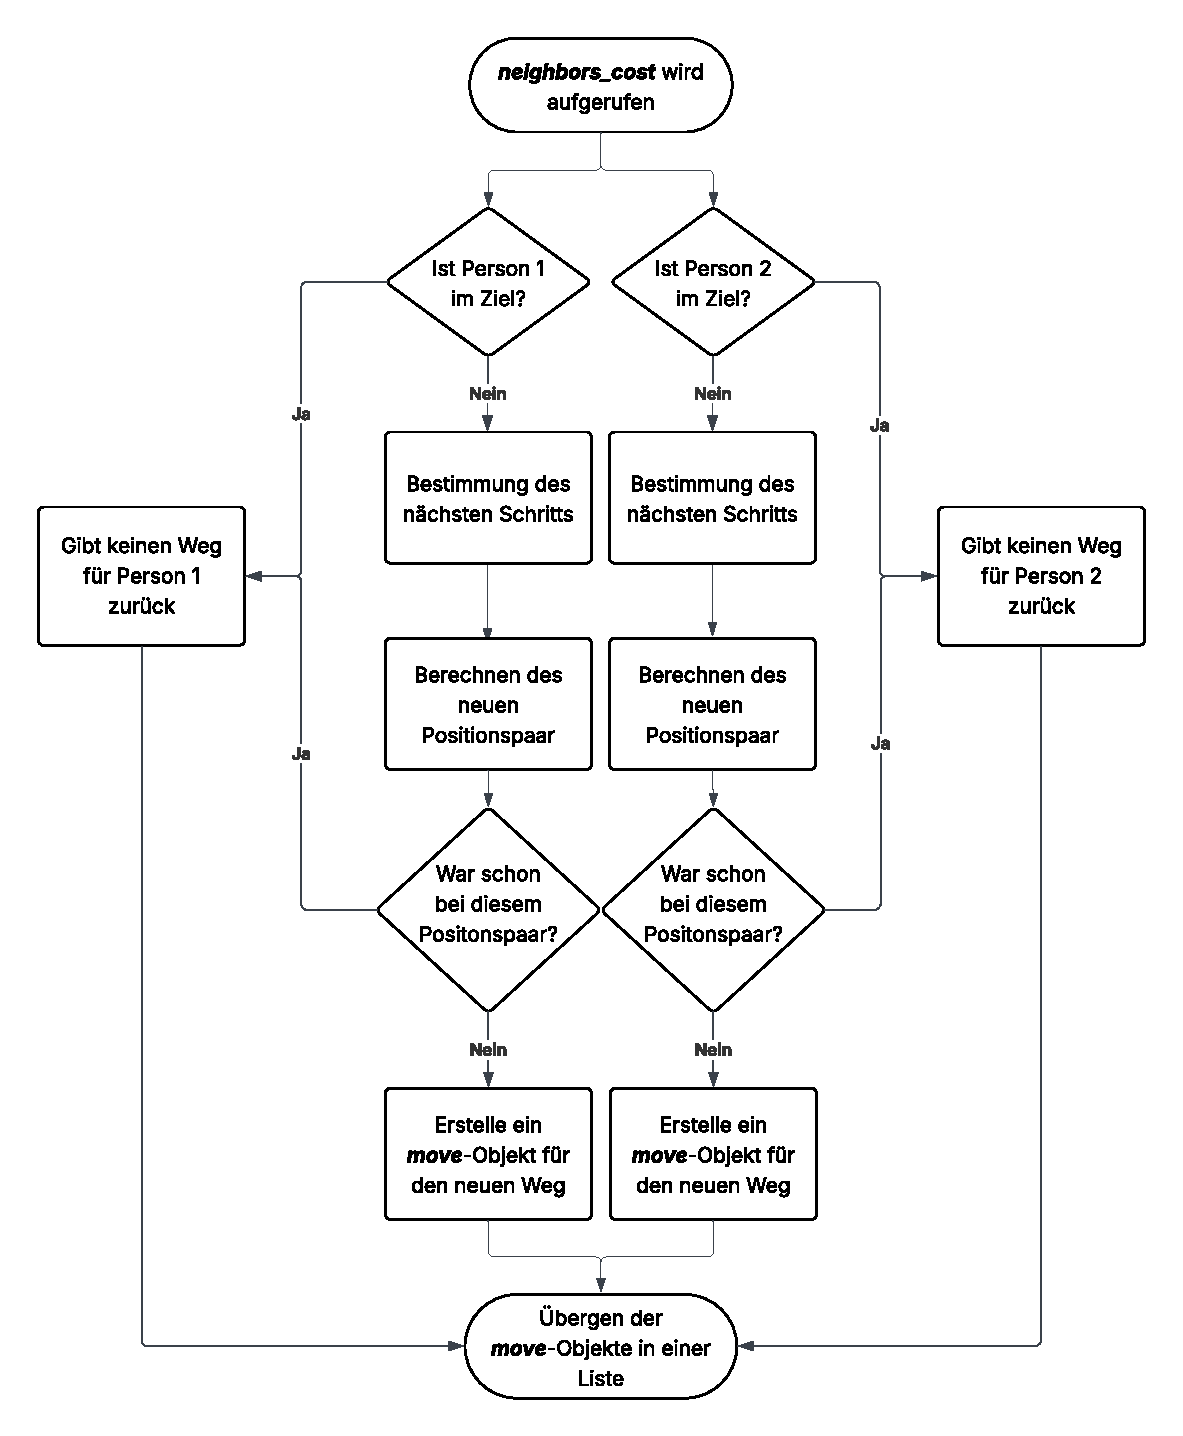
\includegraphics[width=0.8\textwidth]{Simultane Labyrinthe/pdf_src/fluss_diagramm.pdf}
  \caption{$neighbours\_cost$ Flussdiagramm}
  \label{fig:neighbours_cost}
\end{figure}

\clearpage
\section{Laufzeit und Diskussion}
\subsection{Laufzeit}
Wie schon oben erwähnt beeinflussst die Begrenzung $l$, die Laufzeit und Genauigkeit des Algorithmus stark.
\begin{figure}[h]
  \centering
  \begin{minipage}{0.48\textwidth}
    \centering
    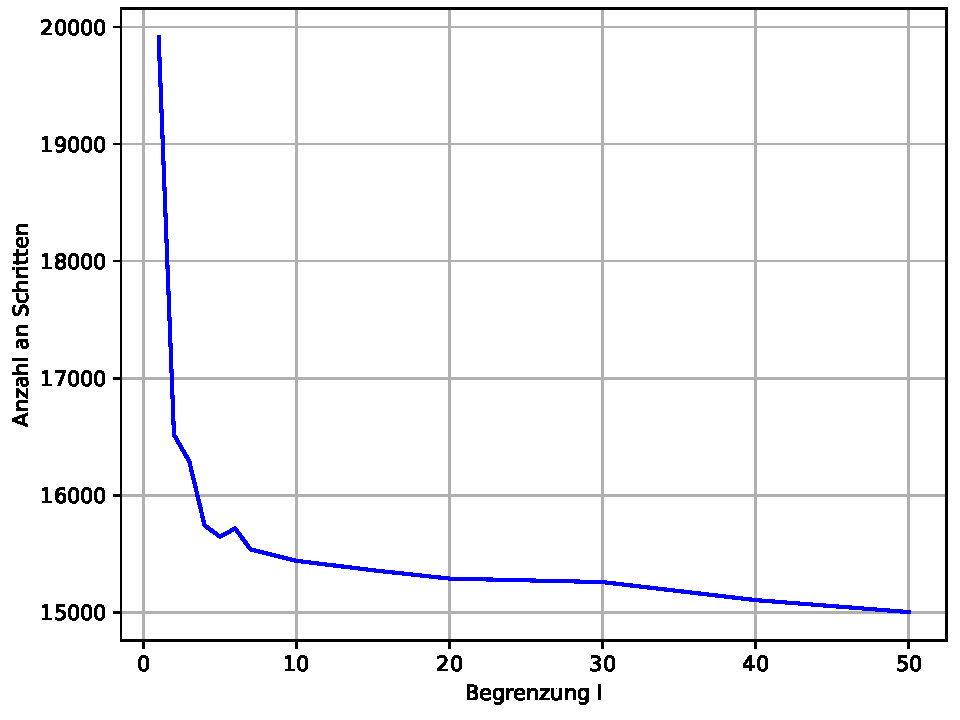
\includegraphics[width=\textwidth]{Simultane Labyrinthe/pdf_src/plotting_schritte_1.pdf}
    \caption{Länge des besten Weges}
    \label{fig:schritte_1}
  \end{minipage}
  \hfill
  \begin{minipage}{0.45\textwidth}
    \centering
    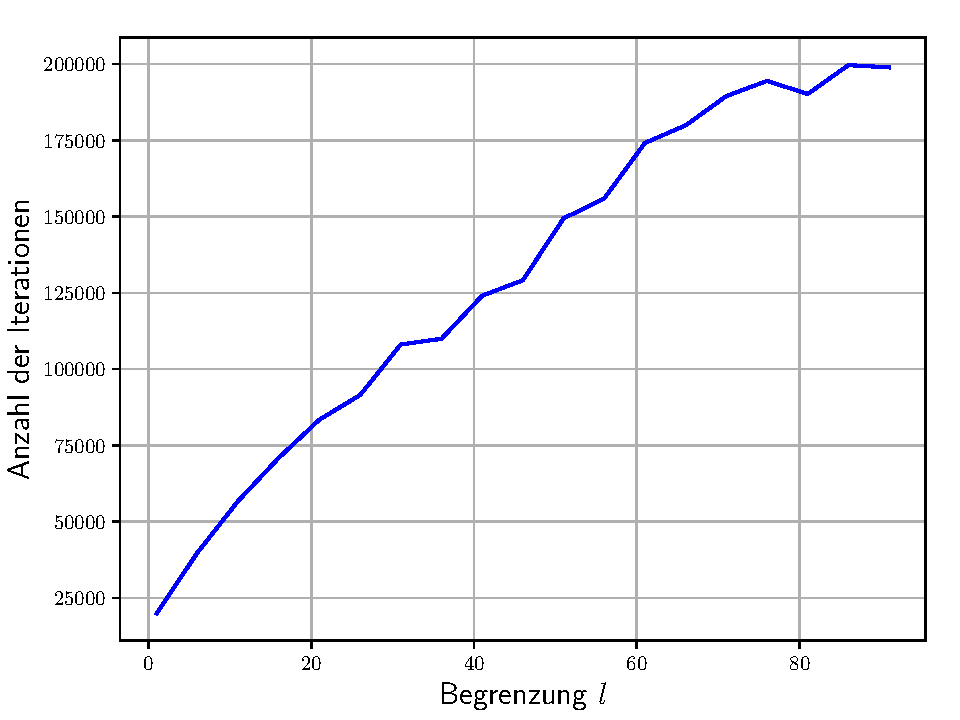
\includegraphics[width=\textwidth]{Simultane Labyrinthe/pdf_src/plotting_laufzeit_1.pdf}
    \caption{Anzahl der Iterationen}
    \label{fig:laufzeit_1}
  \end{minipage}
\end{figure}

Abbildung \ref{fig:schritte_1} zeigt, aus wie vielen Schritten der gefundene Lösungsweg besteht - in Abhängigkeit von $l$.
Abbildung \ref{fig:laufzeit_1} stellt die Anzahl an Iterationen dar, die zur Bestimmung des Lösungsweg benötigt wurden - in Abhängigkeit von $l$
\\

Auffällig ist, dass der Graph in Abbildung \ref{fig:schritte_1} stark exponentiell fällt und sich dabei zunehmend dem optimalen Weg annähert.
Der Graph in Abbildung \ref{fig:laufzeit_1} hingegen entspricht einer langsam ansteigenden Logarithmusfunktion.
\\
Die maximale Anzahl an Iterationen kann wie folgt berechnet werden:
\begin{equation}
  l\cdot(2c_1+c_2)
  \label{max_iterationen}
\end{equation}
wobei:\\
- $c_1$ die Kosten vom Startpunkt aus der Kostenmatrix 1 sind\\
- $c_2$ die Kosten vom Startpunkt aus der Kostenmatrix 2 sind\\
Der Faktor $2c_1+c_2$ beschreibt die maximale Anzahl an Schritte, aus denen ein möglicher Lösungsweg bestehen kann:
Zunächst erreicht Agent1 das Ziel mit $c_1$ Schritten.
Anschließend läuft Agent2 denselben Weg zurück in ebenfalls $c_1$ Schritten und geht dann selber ins Ziel mit $c_2$ Schritten.
Im schlechtesten Fall geht er für jeden Eintrag in der Liste, also $l$ mal, die maximale Anzahl an Schritten.
Daher ergibt sich die Gleichung \eqref{max_iterationen}, was eine liniare Laufzeit von 
\begin{equation}
  o(l)
  \label{laufzeit}
\end{equation}
ergibt.
\clearpage
Praktisch gesehen entspricht die Laufzeit einer Logarithmusfunktion und ist sehr viel kleiner als die maximale Laufzeit.
\begin{figure}[h]
  \centering
  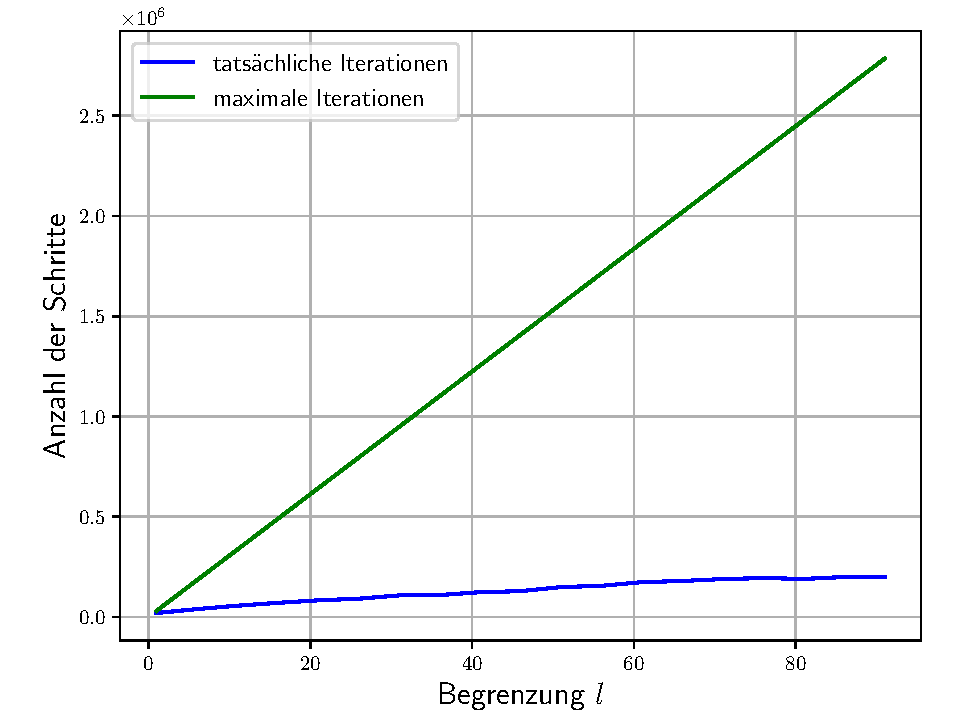
\includegraphics[width=0.5\textwidth]{Simultane Labyrinthe/pdf_src/plotting_max_1.pdf}
  \caption{maximale Iterationen gegenüber tatsächliche Iterationen}
  \label{fig:maximal Laufzeit}
\end{figure}
\\
Der grüne Graph zeigt die maximale Anzahl an Iterationen und der blaue die tatsächliche Anzahl an Iterationen.








\clearpage
\section{Beispiele}
Genügend Beispiele einbinden! Die Beispiele von der BwInf-Webseite sollten hier diskutiert werden, aber auch eigene Beispiele sind sehr gut – besonders wenn sie Spezialfälle abdecken. Aber bitte nicht 30 Seiten Programmausgabe hier einfügen!

\section{Quellcode}
Unwichtige Teile des Programms sollen hier nicht abgedruckt werden. Dieser Teil sollte nicht mehr als 2–3 Seiten umfassen, maximal 10.



\end{document}
